\section{Perturbation-Based Methods}
Perturbation based methods for Visualizing NNs are methods, which compute “the attribution of an input feature (or set of features) by removing, masking or altering them, and running a forward pass on the new input, measuring the difference with the original output” \cite[p.2]{Acona.2018}.
These methods “allow a direct estimation of the marginal effect of a feature” (\cite[p.2]{Acona.2018}), but do not achieve the needed performance when it comes to a higher number of features.
\par
Because of this, there are many new approaches in this field.
Various methods are based on perturbation of input data. In this meta study the focus will be on Prediction Difference Analysis, but multiple other methods will be mentioned and and the current state of research will be explained.


\subsection{LIME}
LIME is another Algorithm that aims to explain the predictions of a NN and is short for “Local Interpretable Model-agnostic Explanations”. It was first introduced by \fcite{Ribeiro.2016} and is freely accessible at https://github.com/marcotcr/lime.
\par
It is applicable to different types of data, like pictures and text and computes the most relevant features of this input. For a picture LIME would output the relevant parts of a picture, for a text the decisive words ín some form of diagram. The explainers correspond with the actual explanation at 90 to 97\%. Multiple examples will be seen in this paper and compared to other methods \cite{Ribeiro.2016}.

\subsection{Occlusion Methods}
Occlusion Methods, otherwise known as Input Masking or Representation Erasure, alter the input by concealing certain parts of the input data and measuring the difference in the output compared to the original output. 
\par
\fcite{Li.2016} use this method for word embeddings. They mask the Pre- or Suffix or other Dimensions of a word and calculate the difference in the output. Like this, the most important dimensions can be found. Interestingly erasure of certain words returns an negative importance score, this means, it improves the decision of the network

\subsection{Contrastive Explanations Method CEM (with Monotonic Attribute Functions)}
The Contrastive Explanations Method was first published by \fcite{Dhurandhar.2018} in 2018 in their paper "Explanations based on the Missing: Towards Contrastive Explanations with Pertinent Negatives".
The CEM approach aims to identify the minimal amount of pixels to justify a classification, called \glspl{pp} pertinent positives\todo{fix}. On the other hand side it identifies the pixels as well, that need to be “turned off” in order to change the classification of the image. These pixels are called \glspl{pn} pertinent negatives. Like this, the most important pixels can be found \fcite{Luss.}. 
\par
“For example, when justifying the classification of a handwritten image of a 3, the method will identify a subset of non-zero or on-pixels within the 3 which by themselves are sufficient for the image to be predicted as a 3 even if all other pixels are turned off (that is, made zero to match background). Moreover, it will identify a minimal set of off-pixels which if turned on (viz. a horizontal line of pixels at the right top making the 3 look like a 5) will alter the classification.” (\fcite{Luss.} p.2)
This example is visualized in figure 2 \fcite{Dhurandhar.2018}.
For the algorithm \fcite{Dhurandhar.2018} found formulas to calculate such PPs and PNs.
\begin{figure*}
    \center
    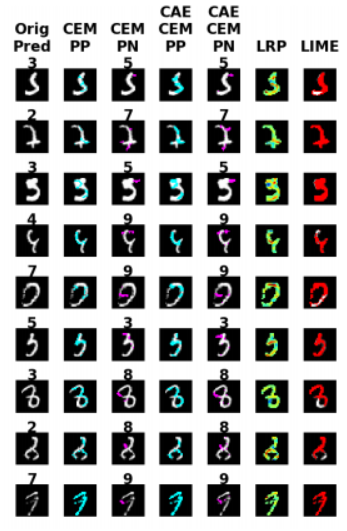
\includegraphics[width=\textwidth/2]{CEM_Numbers}
    \caption{CEM, LRP and LIME applied to a number dataset}
\end{figure*}\todo{add caption}
They applied this method to a dataset of handwritten numbers, like seen in the example\todo{insert picture}. They trained a CNN, which finally reached an accuracy of 99.4\% and then used CEM to visualize these decisions. In addition they used a a convolutional autoencoder (CAE) for some results, which improves this method even further. In figure 3 the output of CEM is visualized. 
\par
To be able to better see the improvements made by this method, LIME and LRP were applied to the same celebrity dataset. It can clearly be seen, that CEM´s results are better understandable for humans.
\begin{figure*}
    \center
    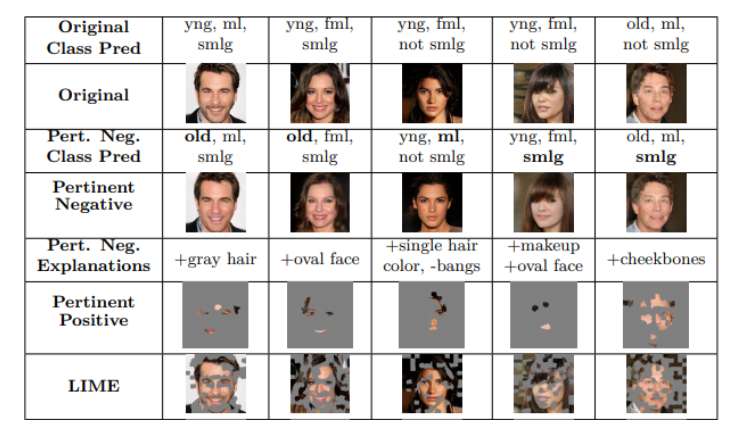
\includegraphics[width=\textwidth]{CEM_Celebs.png}
    \caption{CEM and LIME applied to a celebrity dataset}
\end{figure*}

\fcite{Luss.} improved this method and made it applicable to RGB images.
They found, that “For colored images, PPs offer better direction as to what is important for the classification versus too much direction by LIME (shows too many features) or too little direction by Grad-CAM (only focuses on smiles), while for gray-scale images, neither PPs, LIME, or Grad-CAM are particularly informative versus PNs.“ \fcite[p.7]{Luss.}

\subsection{Prediction Difference Analysis}
The Prediction Difference Analysis was developed 2008 by Robnik-Šikonja and Kononenko and published in the paper “Explaining Classifications for Individual Instances” (\fcite{RobnikSikonja.2008}). They address 3 different types of explanation: instance explanation, model explanation and domain explanation.  Instance explanation aims to explain a “classification of a single instance at model level” \cite[p.2]{RobnikSikonja.2008}. Model explanation measures the averages of explanations over multiple instances and can provide a more general explanation of features and the importance of features values.
\par
Domain explanation is still unknown, but “if the accuracy of the model is high, it should be quite similar to the model explanation.” \cite[p.2]{RobnikSikonja.2008} Firstly they define a model as a function $f : x → f(x)$ which maps instances to numerical values.To calculate the prediction Difference some definitions must be made: An instance x has a value for each attribute $A_{i}$. To now calculate the effect of Ai on x they observe the models prediction for  $f(x\\Ai)$. 
\par
If there is just a minor difference the influence of Ai is small, if there is a major difference the influence is large. The defined formula is: $predDiff_{i} (x) = f(x)− f(x\\Ai)$ .
\par
The difference can be evaluated as 
\begin{itemize}
    \item information difference
        \begin{itemize}
                \item $infDiff_{i}(y|x) = log_{2} p(y|x)−log_{2} p(y|x\\Ai)$
        \end{itemize}
    \item weight of evidence 
        \begin{itemize}
                \item $odds(z) =\frac{p(z)}{p(\={z})} = \frac{p(z)}{(1− p(z)}$
                \item $WEi(y|x) = log_{2} (odds(y|x))−log_{2} (odds(y|x\\Ai))$
        \end{itemize}
    \item difference of probabilities of the output classes
        \begin{itemize}
                \item $probDiff_{i} (y|x) = p(y|x)− p(y|x\\Ai)$
        \end{itemize}
\end{itemize}
\par
The simplest way of computing $p(y|x\\Ai)$ is to replace the value of the attribute Ai with a special but unknown value, knowing, that this approach can lead to incorrectness if the modeling technique does not handle unknown values naturally (naive Bayesian classificator).
To not depend on the model´s implementation they chose an approach, that “simulates the lack of information about Ai with several predictions”\cite[p.4]{RobnikSikonja.2008}.
\par
For  nominal attributes they replace the actual value $A_{i} = a_{k}$ with all possible values for $A_{i}$ and weight the prediction by the prior probability of the value: 
\begin{description}
    \item $p(y|x\\Ai) = \sum_{s=1}^{m_{i}} p(A_{i} = a_{s} | x\\A_{i})p(y|x ← A_{i} = a_{s}) $
    \item $p(y|x\\Ai) = \sum_{s=1}^{m_{i}} p(A_{i} = a_{s})p(y|x ← A_{i} = a_{s}) $
\end{description}

It should be kept in mind, that different instances predict different values, so the explanation differs from instance to instance. Additionally the explanation is dependent on the model, so if the model is incorrect, the explanation will reflect that. The same goes for class dependency, different classes will lead to different explanations.
The results of the prediction difference can then be visualized in a diagram. This special method is called explainVis. The example shown is based on the Titanic data set and predicts the probability of survival of the person based on travelling class, age and gender.
\par
The information difference is shown on the horizontal axis. Weight of evidence and difference of probabilities produce similar graphs and explanations but differ in scale. On the vertical axis the name of the attribute can be found on the left side and the values for chosen instances on the right side. The class probability 
$p(y|x)$
 which was calculated by the model is reported on the top.
The length of the dark grey bar corresponds to the influence of the feature according to the information difference. Positive influence is given on the right-hand side and negative on the left-hand side. The light grey bar represents the influence across all instances for the corresponding attribute value. This shows the overall trend for the feature.
\par
\fcite{Zintgraf.2017} refined this approach even further. They found, that removing one feature at a time is not enough, because a complex neural network is robust to just one unknown feature, like a pixel in an image. Therefore multiple features should be removed at a time so see an impact. In \cite{Zintgraf.2017} they are using images to demonstrate this. They choose patches of connected pixels as their feature sets. The patches have a size of k x k pixel or for an rgb image k x k x 3. Because they use a sliding window style the patches overlap, which makes it possible, to define the individual pixels impact. Depending on the size of the window different results can be found 
\par
It is visible, that a small window does not show the intended results. On the other hand a large window leads to a blurry and not clearly understandable image as well. Therefore observing the results and varying the window size is necessary .like it can be seen in figure 4 (\cite{Zintgraf.2017}). 
\begin{figure*}
    \center
    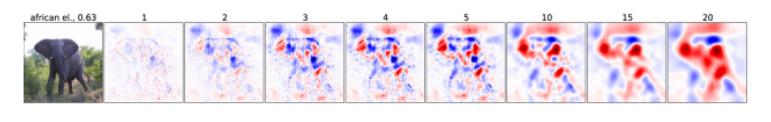
\includegraphics[width=\textwidth]{PredictionDifferenceAnalysis}
    \caption{Prediction Difference Analysis with different window sizes}
\end{figure*}

\subsection{Anchors}
Anchors were introduced in 2018 by \fcite{Ribeiro.2018} and can also be referred as if-then rules. They are rules, that “sufficiently “anchors” the prediction locally – such that changes to the rest of the feature values of the instance do not matter” (\cite[p.1]{Ribeiro.2018}). This means, the values of other features are not important if an anchor exists, because the prediction will always be the same. In their paper they apply these anchors to tabular, text and image datasets.
\par
Like in the prediction difference analyses the model is defined as  
$f(x) → y$. 
An instance x ist perturbed by a “perturbation distribution” $D_{x}$ (from now on D). The perturbations D should be in an interpretable form. A is a set of rules, which is applicable on x. $A(x)$ returns true (1), if all feature predicates are true for instance x.
If 
$A(x) = 1$
 and “A is a sufficient condition for $f(x)$ with high probability” \cite[p.2](Ribeiro.2018) (bigger than τ), then A is an anchor. Formally this can be described with 
\par
$E_{D(z|A)} [\mathbb{1}_{f(x)=f(z)}] ≥ τ, A(x) = 1$
 \par
An example of anchors for texts can be seen in figure 5. What LIME is, is explained in section LIME. In the figure you can see possible Anchors: e.g. for anchor A = {“not”, “bad”} the model will predict “positive “ with a probability of more than τ. If one or more of these words are missing, there is no anchor and with that it is not certain, what the output will be.
The paper presents two different ways for finding those anchors: a bottom-up construction or a Beam-Search.
\begin{figure*}
    \center
    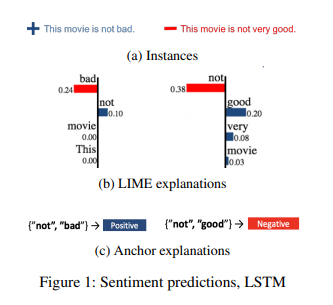
\includegraphics[width=\textwidth/2]{Anchor}
    \caption{possible Anchors for textual data}
\end{figure*}\todo{add caption}
\par
With the bottom up search they try to find a rule with the highest estimated precision, and like this the shortest anchor. This anchors tend have a high coverage and are easily understandable for humans. 
The downside of this approach is, that this greedy strategy is only able, to find one anchor at a time and the coverage is just negligibly.
The beam search aims “to identify amongst many possible anchors the one that has the highest coverage” \cite[p.5]{Ribeiro.2018}. This is done similar to the greedy approach. First all candidate rules are computed, then the best rules are selected.

\subsection{Activation Maximization}
Activation Maximization aims to find an input, which maximizes the output score for a certain class. It was first published in a technical report by \fcite{Erhan.2009} in 2009. They restricted themselves to find the image of the dataset they had, that maximizes the feature.
\par
\fcite{Le.2012} refined this approach in 2012 and not only found the input images with the highest stimuli, but were able to compute an own picture (picture) \cite{Le.2012}.
\par
There are multiple frameworks that can generate such pictures. A well-known method was developed by Zeiler and Fergus in 2014 called DeConvNet \cite{Zeiler.2014}. They mapped features to pixels, instead of the other way around:
“To start, an input image is presented to the convnet and features computed throughout the layers. To examine a given convnet activation, we set all other activations in the layer to zero and pass the feature maps as input to the attached deconvnet layer. Then we successively (i) unpool, (ii) rectify and (iii) filter to reconstruct the activity in the layer beneath that gave rise to the chosen activation. This is then repeated until input pixel space is reached.” \cite[p.820]{Zeiler.2014}.
\par
\fcite{Nguyen.2016} achieved this in 2016 by starting from a random image and calculating via backpropagation how each pixel influences the output. Multiple studies have shown, that this can lead to unrealistic images. To improve in this point a general concept of a natural image must be learned by the NN. Therefore Nguyen et al. are using image generator networks. They conclude, that they can understand better, which features a NN has learned exactly with this method \cite{Nguyen.2016}. 
\par
In figure 6 the learned feature "face" is demonstrated. On the upper half the actual input images are shown, which activate the neuron the most. On the bottom the generated image is shown.
\begin{figure*}
    \center
    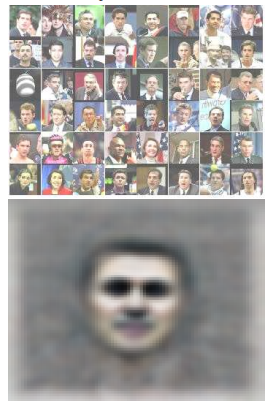
\includegraphics[width=\textwidth/2]{ActivationMaximization}
    \caption{Inputs, that activate the "face-neuron" the most.
    Top: actual input images 
    Bottom: via backpropagation found input}
\end{figure*}\todo{add number?}